\lecture{3. They Shall Be My People}{03}

\section{Introduction}

\begin{frame}
\frametitle{Tebow-ing}
\begin{center}
	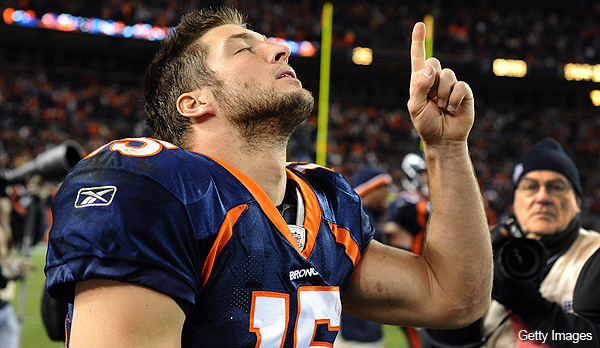
\includegraphics[width=\textwidth]{figures/footballPoint.jpg}
\end{center}

\note{09:30}
\note[item]{Sometimes we sneer at the guys like Tim Tebow who give God the glory when they make a touchdown.}
\note[item]{We say things like, `God isn't concerned about their football game.', or, `What about the other team?'}
\note[item]{But there's still a piece of me that admires them, because, even if they are a bit shallow, at least at some level they accept two facts\ldots}
\note[item]{Whatever advantages or achievements they have in sports, , they come from God.}
\note[item]{They believe that God is on their side, helping them.}
\note[item]{God \emph{is} on our side.}
\note[item]{Do we believe in the advantages that provides?}
\note[item]{Today we examine what it means to be `God's people'}
\end{frame}

\begin{frame}
\frametitle{God wants a relationship with people}
\framesubtitle{Jeremiah 31:31-34}
	\keyversehiglight{they shall be my people}

\note{09:32}
\note[item]{Last week was about how we should be proud of God.}
\note[item]{This week is about how God is proud of us.}
\end{frame}

\begin{goals}
\goal Recognize that God wants a people who choose Him voluntarily
\goal Understand that God always provides a way and a reward for His people
\goal Appreciate how unique and special a Christian's relationship with God is

\note{09:33}
\note[item]{Some tough passages today.}
\end{goals}

\section{God wants volunteers}

\begin{frame}
\frametitle{God invites, but doesn't coerce}
\framesubtitle{Matt 22:1-14}
\begin{center}

\includegraphics[width=\textwidth]{figures/volunteer.jpg}
\end{center}
All the original guests to the feast had to do was show up.

\note{09:35}
\note[item]{He's offering them something for the feast.  All they have to do is show up.}
\end{frame}

\begin{frame}
\frametitle{No impostors allowed}
\framesubtitle{Matt 22:1-14}
\begin{columns}[T]
\begin{column}{0.4\textwidth}
\begin{center}

\includegraphics[width=\textwidth]{figures/imposter.jpg}
\end{center}
\end{column}
\begin{column}{0.6\textwidth}
\begin{itemize}
\item You've got to have the right clothes to be part of the feast.
\item Sincerity and truth in thought and action is a requirement
\item There's severe consequences for hypocrisy.
\end{itemize}
\end{column}
\end{columns}

\note{09:38}
\note[item]{Matt. 7:21 Not everyone who says to me Lord, Lord will enter the kingdom of heaven but he who does the will of my father.}
\end{frame}

\begin{frame}
\frametitle{Many are called few are chosen.}
\framesubtitle{Matt 22:1-14}
\begin{center}

\includegraphics[height=0.7\textheight]{figures/different.jpg}\\
The people of God have to embrace being different.\\
You volunteered for this.
\end{center}

\note{09:40}
\note[item]{God's people will be special because He chose them.}
\note[item]{But, also because they chose Him.}
\note[item]{And, we're not different because we're somehow innately better than the world.}
\note[item]{On the contrary, the people who are called in the parable were the low people in society not the elites.}
\end{frame}

\begin{frame}
\frametitle{You can always choose not to.}
\framesubtitle{Matt 22:1-14}
\begin{center}

\includegraphics[width=\textwidth]{figures/iQuit.jpg}
\end{center}

\note{09:42}
\note[item]{If being a Christian is not what you want, then you can choose to go back to the world}
\note[item]{When we were considering dropping the Sunday evening service in favor of our current format some people were adamant that a distinction be made between the `required' Sunday AM service and the `optional' Sunday afternoon service.}
\note[item]{\emph{All} services are optional!}
\note[item]{We're here because we volunteered.}
\note[item]{So, we should act like we want to be here.}
\end{frame}

\section{God provides for His people}

\begin{frame}
\frametitle{God will always provide for His people}
\framesubtitle{Ezekiel 37}
\begin{center}
	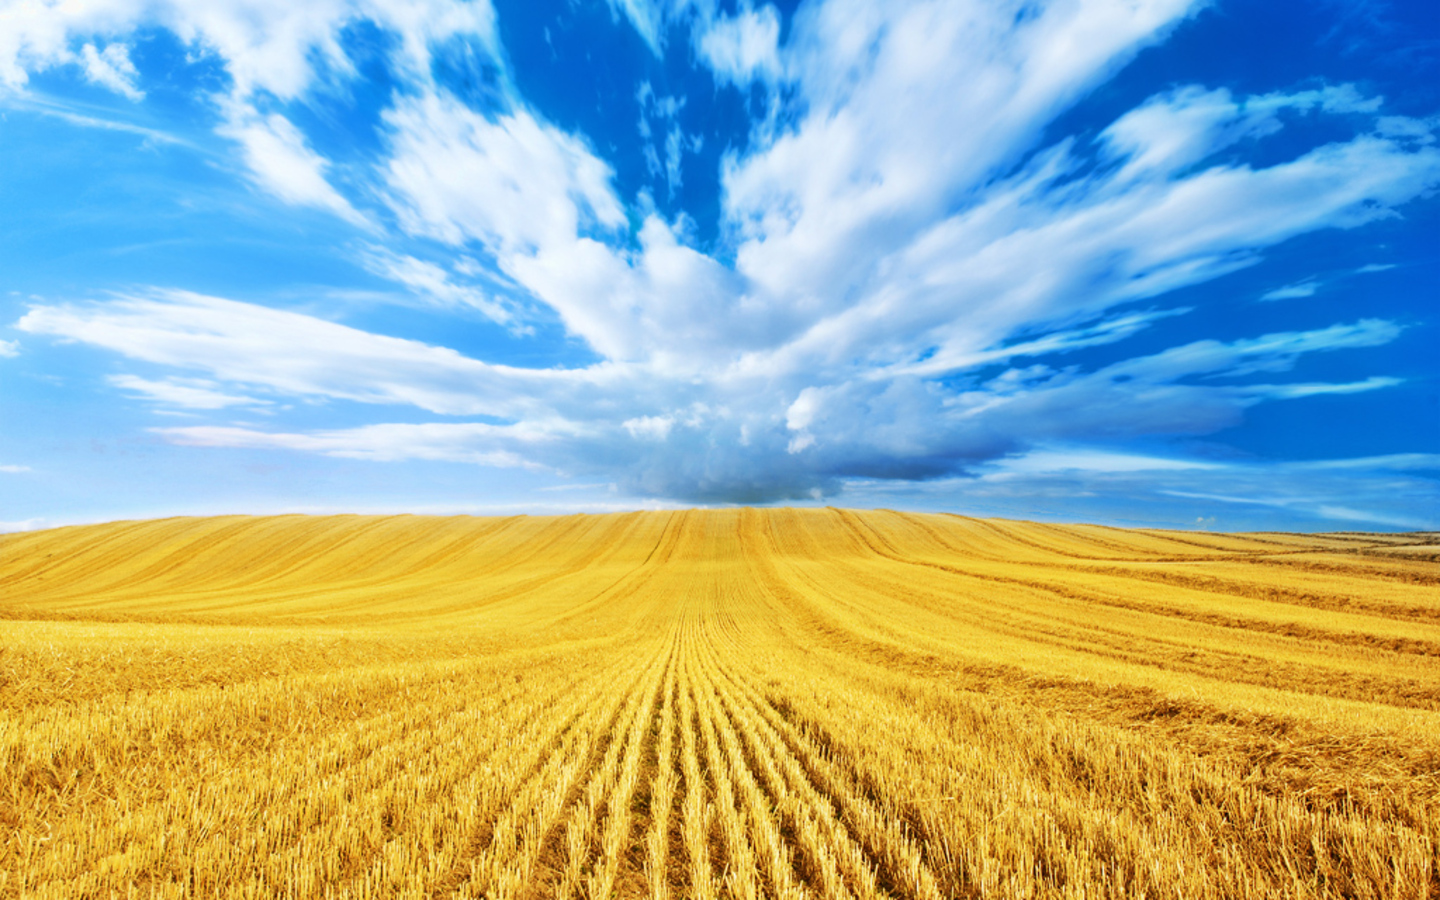
\includegraphics[width=0.6\textwidth]{figures/abdundance.jpg}
\end{center}
\begin{description}
\item[1-14] The Valley of the Dry Bones -- God will resurrect His people
\item[15-28] The Joined Stick -- God will give His people an everlasting possession.
\end{description}

\note{09:44}
\note[item]{Ezekiel was a prophet while Judah was in Babylonian captivity.}
\note[item]{In context it seems like the people had given up hope that God would ever bless them again.}
\note[item]{These two connected prophecies talk about what God is going to do for His People}
\note[item]{God's people will win!}
\note[item]{Dry Bones - God will resurrect His people}
\note[item]{Joined Stick - God will give them an everlasting possession.}
\end{frame}

\begin{frame}
\frametitle{God will resurrect His people}
\framesubtitle{Ezekiel 37:1-14}
\begin{columns}[T]
\begin{column}{0.4\textwidth}
	\begin{center}
	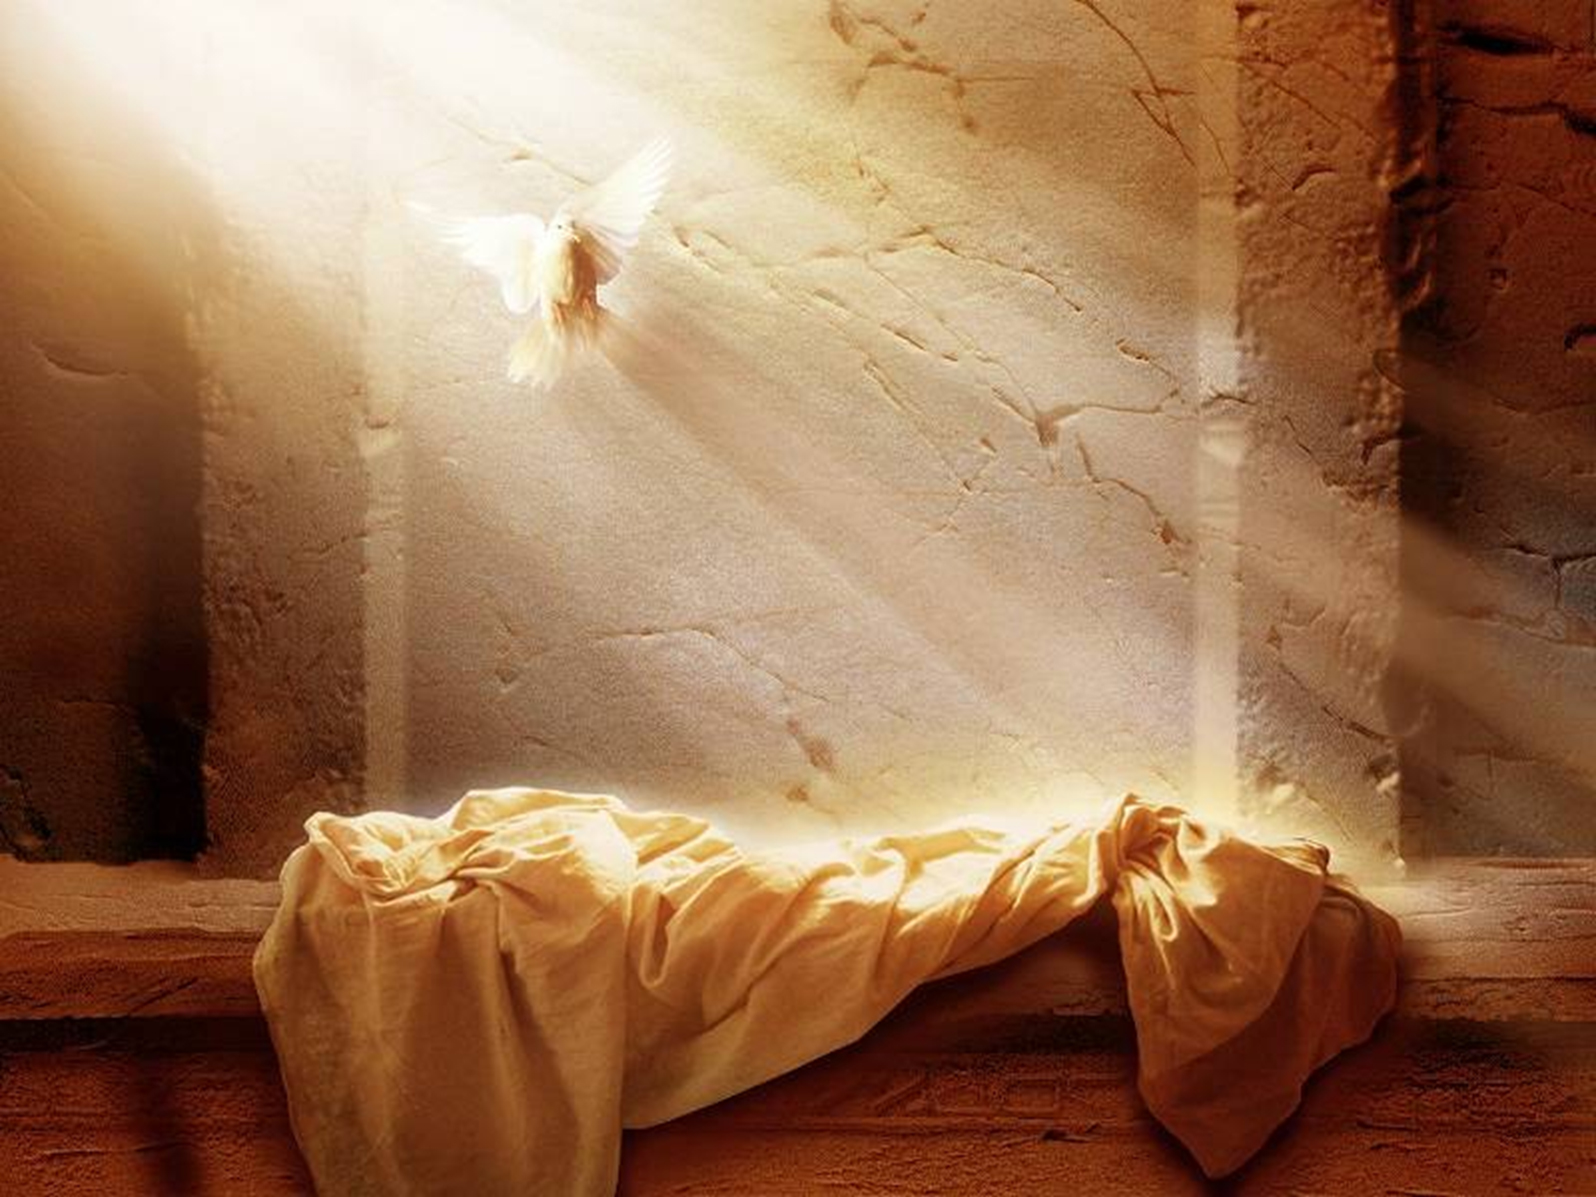
\includegraphics[width=\columnwidth]{figures/resurrection.jpg}
	\end{center}
\end{column}
\begin{column}{0.6\textwidth}
This is one of the few passages in the Old Testament that directly refers to the resurrection from the dead.\\~\\
With a New Covenant perspective we see three resurrections eluded to in this prophecy:
	\begin{itemize}
	\item Physical Israel would return from captivity.
	\item Spiritual renewal in the Holy Spirit under the New Covenant
	\item Bodily resurrection from the dead at the last day
	\end{itemize}
\end{column}
\end{columns}

\note{09:46}
\note[item]{There are really 3 ways this prophecy is fulfilled.  And three ways we're resurrected from the dead}
\note[item]{Vs. 11 says explicitly that the bones are the whole house of Israel.}
\note[item]{Says God will put His Spirit within them}
\note[item]{Land must be figurative.  This is premellinialism.}
\note[item]{They will no longer be a divided kingdom.  But, Ezekiel was prophesying during captivity after Israel had already been taken away.}
\note[item]{Clearly this has to be Christians.}
\note[item]{The dead shall live and you shall know that I am the Lord}
\note[item]{Resurrection is a key feature of the people of God.}
\end{frame}

\begin{frame}
\frametitle{God will give His people an everlasting possession}
\framesubtitle{Ezekiel 37:15-23}
\begin{center}
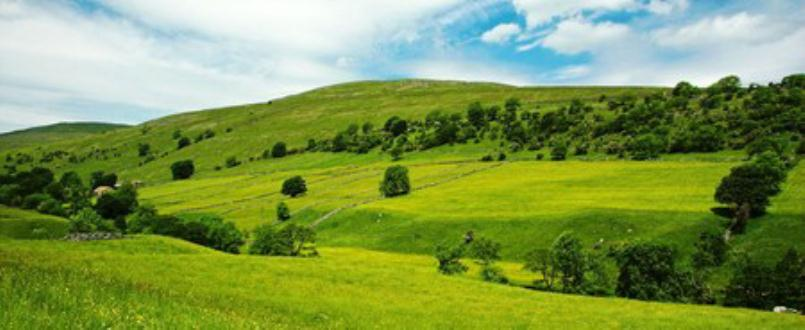
\includegraphics[width=0.8\textwidth]{figures/land.jpg}
\end{center}
\begin{itemize}
\item ``I will \ldots bring them to their own land.''
\item ``Make them one nation''
\item ``One king''
\item ``My dwelling place shall be with them''
\item ``I will be their God and they shall be my people''
\end{itemize}

\note{09:50}
\note[item]{The people of God always have a land, a place, a possession.}
\note[item]{The prophecy must refer to spiritual Israel, because restoration of the physical Northern tribes never did occur.}
\note[item]{With all this emphasis on the land, it's no wonder that the people of Israel had a hard time accepting Jesus, and why the physical restoration of Israel is a key doctrine for premellinialists.}
\note[item]{They were thinking that God had forgotten them.}
\note[item]{That times would never get better.}
\end{frame}

\begin{frame}
\frametitle{God's people still have a promised land}
\framesubtitle{Hebrews 11:13-16}
13 These all died in faith, not having received the things promised, but having seen them and greeted them from afar, and having acknowledged that they were strangers and exiles on the earth. 14 For people who speak thus make it clear that they are seeking a homeland. 15 If they had been thinking of that land from which they had gone out, they would have had opportunity to return. 16 But as it is, they desire a better country, that is, a heavenly one. Therefore God is not ashamed to be called their God, for he has prepared for them a city.

\note{09:54}
\note[item]{Yes, Abraham was promised a physical land, but it was also a spiritual land.}
\note[item]{The faithful from times past looked forward to the spiritual land, not the physical land.}
\note[item]{We have that same promised land -- entrance into the kingdom of God, and, ultimately, heaven}
\end{frame}

\section{God's people are special}

\begin{frame}
\frametitle{The Lord made Israel special}
\framesubtitle{Deut. 10:12-22}
\begin{columns}[T]
\begin{column}{0.5\textwidth}
\begin{center}

\includegraphics[width=\columnwidth]{figures/uniqueFish.jpg}
\end{center}
\end{column}
\begin{column}{0.5\textwidth}
\begin{itemize}
\item No one else got the benefits that Israel did.
\item No one else had the requirements that Israel did.
\end{itemize}
\end{column}
\end{columns}

\note{09:56}
\note[item]{Same verse quoted in Luke 10 last week about loving the Lord}
\note[item]{God selected you above all peoples.  As a result, serve Him.}
\end{frame}

\begin{frame}
	\frametitle{The Lord made Christians special}
	\framesubtitle{I Peter 2:9-10}
	\begin{columns}[T]
	\begin{column}{0.5\textwidth}
		\begin{center}
		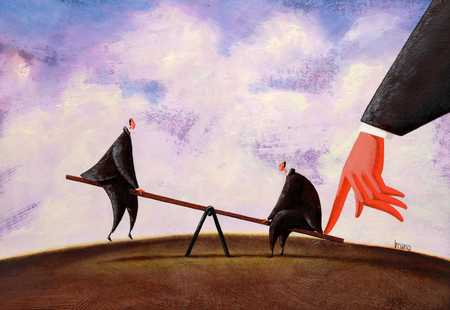
\includegraphics[width=\columnwidth]{figures/unfairAdvantage.jpg}
		\end{center}
	\end{column}
	\begin{column}{0.5\textwidth}
		\begin{itemize}
		\item We are a chosen race (like Israel).
		\item We are a royal priesthood (like Judah and Levi put together!).
		\end{itemize}
	\end{column}
	\end{columns}
	
\note{09:58}
\note[item]{The Israelites were chosen first}
\note[item]{We weren't a people until God gave us the opportunity.}
\note[item]{Investment bankers usually come from rich families.}
\note[item]{Starting out wealthy has its advantages}
\note[item]{This passage reminds us that we're the privileged ones.}
\end{frame}

\begin{frame}
\frametitle{God adopts us as sons}
\framesubtitle{Romans 8:12-17}
\begin{columns}[T]
\begin{column}{0.5\textwidth}
	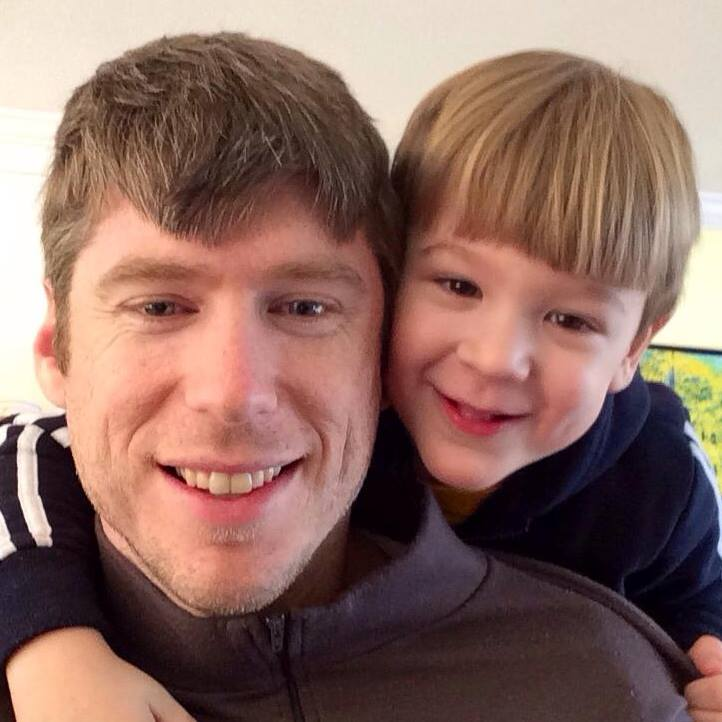
\includegraphics[width=\columnwidth]{figures/toddAndEzra.jpg}
\end{column}
\begin{column}{0.5\textwidth}
	\begin{itemize}
	\item ``Abba, Father'' reveals the closeness we have with God.
	\item We are heirs with Christ.
	\item We will be glorified with Christ.
	\end{itemize}
\end{column}
\end{columns}

\note{10:00}
\note[item]{You look at that picture and think, `Ah, cute'}
\note[item]{I look at that picture and see something completely different -- My son}
\note[item]{That's what `Abba, Father' means}
\note[item]{\emph{What are we heirs of?}  The everlasting kingdom prophesied in Ezekiel 37.}
\note[item]{Some of those blessings we receive now (\emph{e.g.}, entrance into the kingdom)}
\note[item]{Some of those blessings are yet to be revealed (\emph{e.g.}, resurrection from the dead).}
\end{frame}

\begin{frame}
\frametitle{The Lord is with His people from start to finish}
\framesubtitle{Romans 8:28-30}
\begin{columns}[T]
\begin{column}{0.4\textwidth}
	\begin{center}
	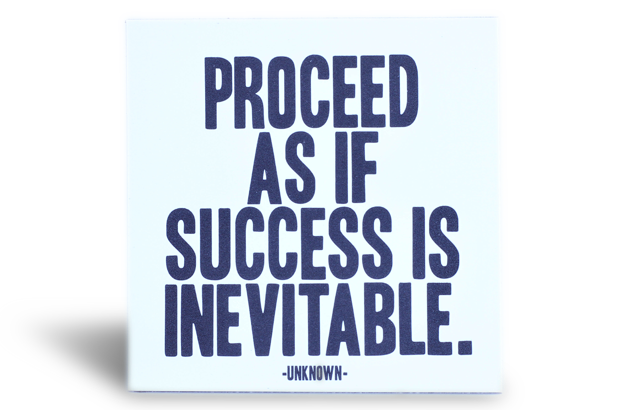
\includegraphics[width=1.3\columnwidth]{figures/success.png}
	\end{center}
\end{column}
\begin{column}{0.6\textwidth}
\begin{itemize}
	\item This passage should encourage us, not simply generate theological discussions.
	\item God's preparations for His people started before time.
	\item God's support of His people will continue through the end of time. 
\end{itemize}
\end{column}
\end{columns}

\note{10:05}	
\note[item]{\emph{Below is a prepared answer if I'm asked about predestination}}
\note[item]{Calvinists misunderstand the sovereignty of God.}
\note[item]{I have no issue with God knowing what happens in the future or even knowing ahead of time those who will be lost or saved.}
\note[item]{God knew ahead of time the poor decisions people would make and what the outcome of those decisions would be (\emph{e.g.}, Rom. 9, Esau, Pharaoh, Judas, Peter).}
\note[item]{Foreknowledge is not causation, however.}
\note[item]{God does not `select' people apart from their own decisions}
\note[item]{Calvinists assume that our decisions are \emph{totally} driven by either our sinful human nature (over which we have no control) or the miraculous influence of the Holy Spirit (for salvation).}
%\note[item]{Sociologists have the same problem.  Their whole field  is predicated on the assumption that your environment is the sole determinants of your choices.}
\note[item]{This contradicts Matt 22, which we've already discussed.}	
\end{frame}

\section{Review}

\begin{frame}
\frametitle{They shall be my people}
	\begin{itemize}
		\item God wants volunteers
		\item God makes a way for His people
		\item God gives His people eternal possessions
		\item God's people are special
		\item The best days are still ahead of us
	\end{itemize}

\note{10:10}
\note[item]{You are special.}
\note[item]{Act like it.}
\note[item]{Better days are ahead, because you are God's people.}
\end{frame}
